\documentclass[../main.tex]{subfiles}

\begin{document}
    
\chapter{Optimal Sector Universes}

\section{Backtesting Results}

In pervious chapter we develop a Python packege to implement the backtesting of sector universes. Then we do backtesting with sector universes we gennerate from Chapter 5 and collect data for 60 sector universes. We plot graphs of cumulative ETF restructuring turnover, cumulative portfolio rebalancing turnover, portfolio return and portfolio Sharpe Ratio over time respectively. 

% image may list here or in appendix
\begin{figure}[H]
    \includegraphics{}
    \caption{}
    \label{}
\end{figure} 

\section{Optimal Universes Selection}

The next step is to select the optimal universe from 60 sector universes under different criteria. For ETF restructuring turnover and portfolio rebalancing turnover, which represent the cost in backtesting, less is better. For portfolio return and Sharpe Ratio, which represent the gain in backtesting, higher is better. Thus, optimal sector universe for turnover is the one that has lowest cumulative turnover. optimal sector universe for return or Sharpe Ratio is the one that has highest return or Sharpe Ratio. The results are list below: 

\begin{itemize}
	\item Minimum cumulative ETF restructuring turnover: Single Linkage; 5 Sectors
	\item Minimum cumulative portfolio rebalancing turnover: Single Linkage; 5 Sectors
	\item Maximum portfolio return: Complete Linkage; 9 Sectors
	\item Maximum portfolio Sharpe Ratio: Complete Linkage; 16 Sectors
\end{itemize}
    
Here are the visualizations of optimal sector universes with different criteria:

\begin{figure}[H]
    \centering
    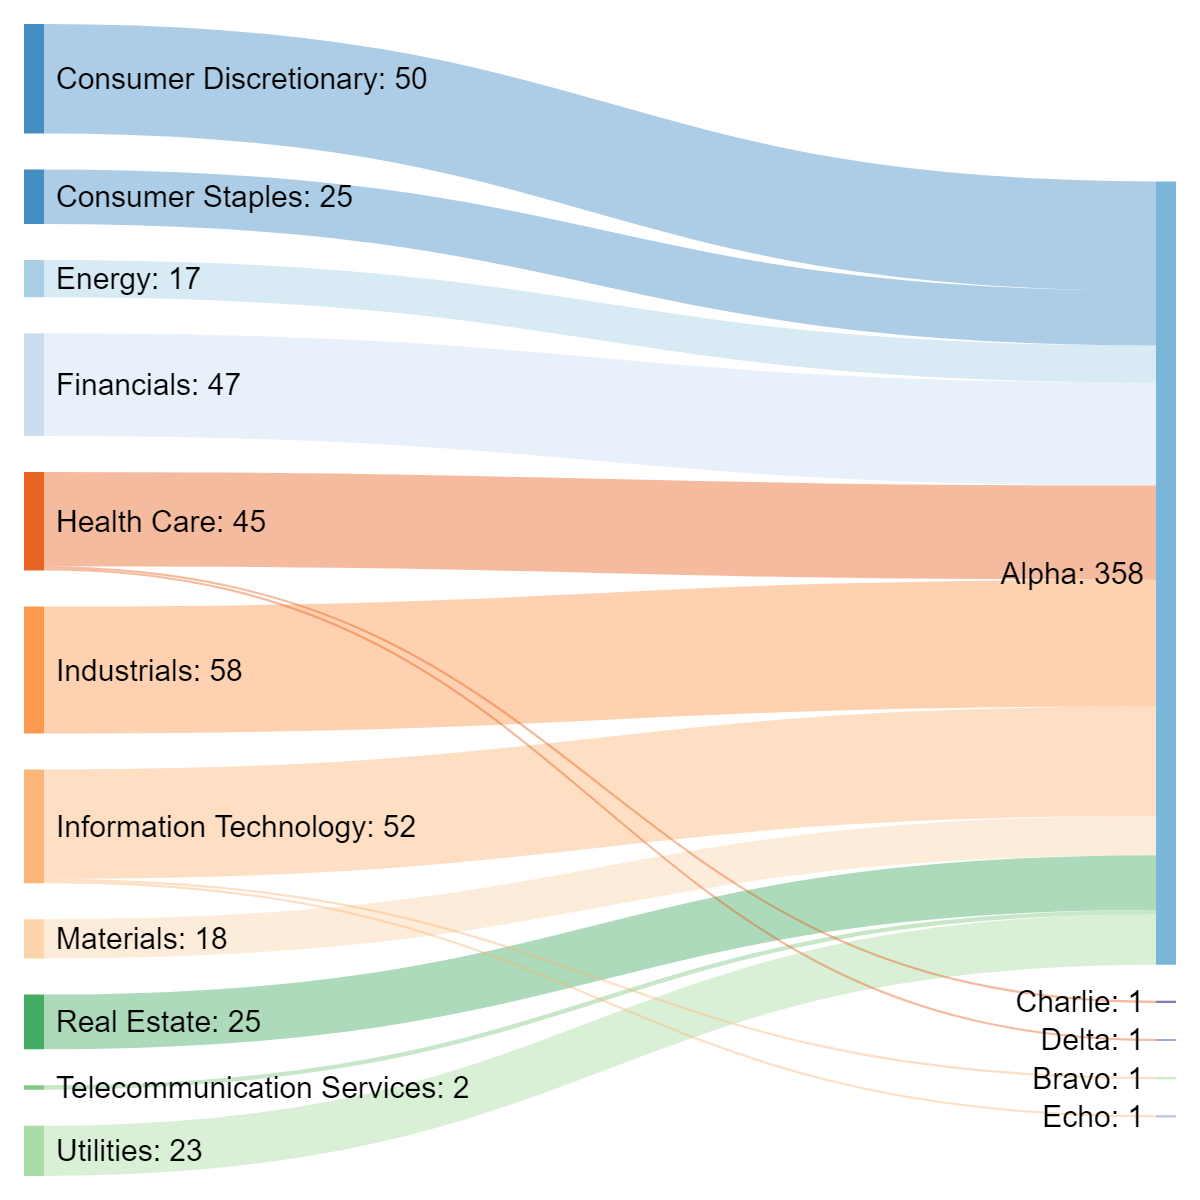
\includegraphics[scale=0.2]{images/single_2017_5.png}
    \caption{Minimum Turnovers Sector Universe}
    \label{fig:optimal_sector_universes:min_turnover}
\end{figure} 

\begin{figure}[H]
    \centering
    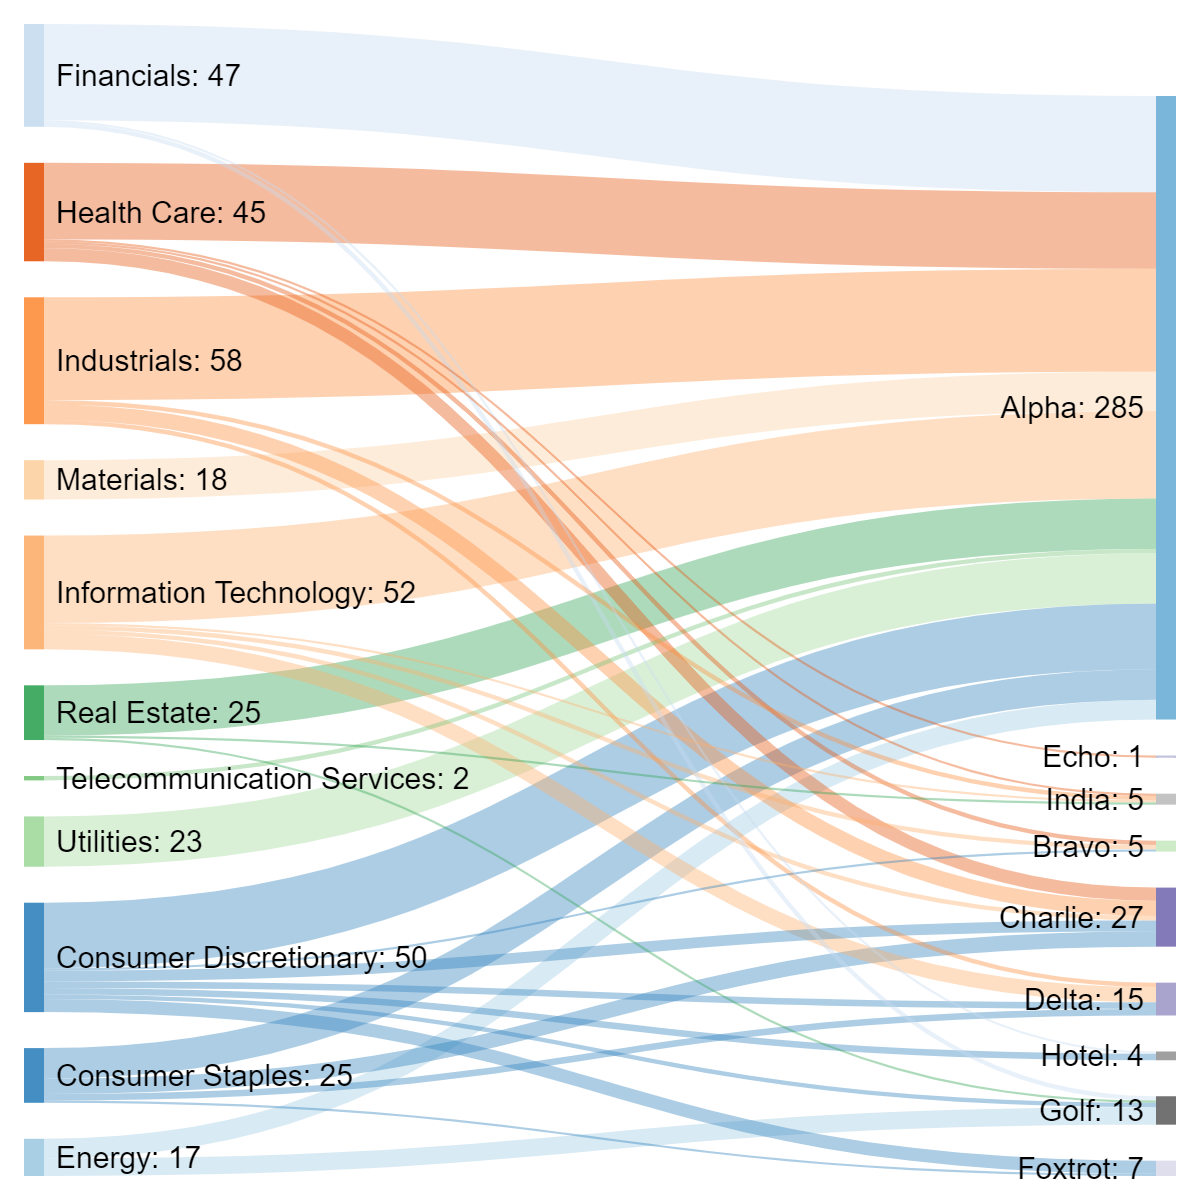
\includegraphics[scale=0.2]{images/complete_2017_9.png}
    \caption{Maximum Portfolio Return Sector Universe}
    \label{fig:optimal_sector_universes:max_return}
\end{figure}

\begin{figure}[H]
    \centering
    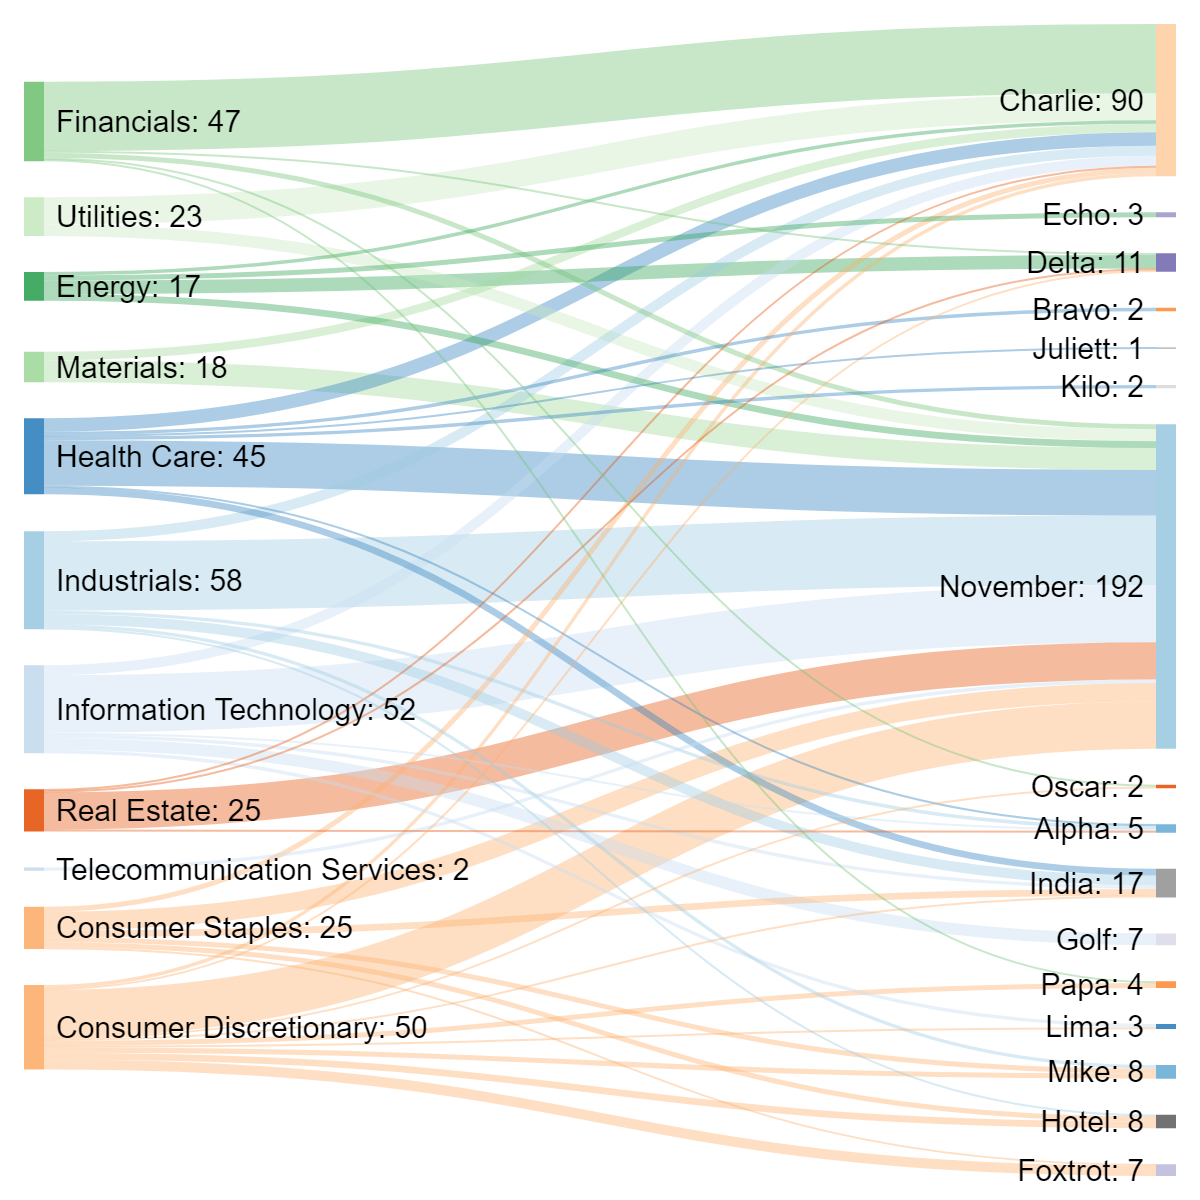
\includegraphics[scale=0.2]{images/complete_2017_16.png}
    \caption{Maximum Portfolio Sharpe Ratio Sector Universe}
    \label{fig:optimal_sector_universes:max_sharpe}
\end{figure}

From the graph of Single Linage and  5 Sectors, we can find that most companies are clustering in one huge sector, and other sectors only contain one individual company. That is the reason why this sector universe has lowest turnovers: since some sectors only contain one company, they do not generate ETF restructuring turnover and low portfolio rebalancing turnover. 

\section{Optimal Universe for Sharpe Ratio}

Since our goal is to evaluate risk-adjusted return of our Learned Sector, we focus on the optimal universe with maximum Sharpe Ratio. Companies from Heaith Care, Information Technology, Consumer Staples and Comsumer Discretionary are separated into different new sectors. Most companies from Financials, Energy and Industrials are classified into same sectors in new sector classification. Also, the phenomenon of one or two "big" sevctors and several "small" sectors coexist exists. 

\end{document}